\documentclass[cn,table]{elegantbook}

\usepackage{tikz}
\usepackage{graphicx}
\usepackage{subcaption}
\usepackage[ruled,linesnumbered,vlined]{algorithm2e}
\usepackage{hyperref}
\usepackage{listings}
\usepackage{interval}
\usepackage{xcolor}
\usepackage{ulem}
\usepackage{wrapfig}

\intervalconfig{%
	soft open fences,
}

\def\figureautorefname{图}
\def\sectionautorefname{小节}

\SetAlgorithmName{算法}{算法}{算法索引}

\renewcommand*{\lstlistingname}{代码}

\title{何老师算法课笔记}
\subtitle{Always be patient, sharp and diligent.}
\author{计卓1801全体}
\institute{华中科技大学}
\date{\zhtoday}
\version{1.8.0}
\logo{logo.png}
\cover{cover.png}

\begin{document}
\maketitle
\tableofcontents
\pagenumbering{arabic}

% add your code here
% \input{src/example.tex}
\input{src/Ln1-AsymptoticOrderGrowth.tex}
\input{src/Tiling-Problem.tex}
\input{src/stable-matching.tex}
\input{src/Ln9-NearestPoints.tex}
\input{src/Ln11-LargeIntegerMultiplication.tex}
\input{src/dynamic-programming-1.tex}
\chapter{字符串编辑距离}

\begin{introduction}
	\item 问题引入
	\item 相关概念
	\item 算法思想
\end{introduction}

\section{问题引入}
如何定义两个字符串的距离呢?ocurrance和occrrence有多大的区别呢?下面我们将讨论两个字符串的距离问题。
\section{相关概念}
\begin{definition}{匹配M}{matching}
	字符串X有$x_1$到$x_n$共n个字符,字符串Y有$y_1$到$y_m$共m个字符。X和Y之间存在一个匹配M,其满足:$if (i,j) \in M, (l,k)\in M, i<l iff j<k$。
\end{definition}

%距离代价:

%$\alpha_{xy}$ :两个不同的字符x和y相匹配的代价,则$\alpha_{xy}=0$.

%$\delta$ :每存在一个没有被选择的字符就会多一个$\delta$.

%总距离代价:所有$\delta$ 和 $\alpha$ 的和。

\begin{definition}{距离代价}{penalty}
	$\alpha_{xy}$:两个不同的字符x和y相匹配的代价,则$\alpha_{xy}=0$.
	
	$\delta$:每存在一个没有被选择的字符就会多一个$\delta$.
	
	总距离代价:所有$\delta$ 和 $\alpha$ 的和。
\end{definition}

示例:

\begin{figure}[htb]
	\centering
	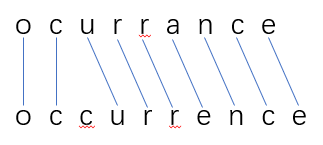
\includegraphics[scale=0.6]{image/connect1.png}
	\caption{字符串匹配}\label{fig:connect1}
\end{figure}
如上图所示,其中的总距离代价为$\alpha_{ae} + \delta$

\section{算法思想}
从后往前推:

bopt (i,j):字符串$x_1,\ldots,x_i$和$y_1,\ldots,y_j$之间的最佳匹配
\begin{equation}
	bopt (m,n)=\begin{cases}
		bopt(m-1,n-1)+\alpha_{x_m y_n} & \text{$x_m$和$y_n$ 相连} \\
		bopt (m-1,n)+\delta            & \text{$x_m$跳过}         \\
		bopt (m,n-1)+\delta            & \text{$y_n$跳过}
	\end{cases}
\end{equation}

从前往后推:

fopt (i,j):字符串$x_i,\ldots,x_m$
和
$y_j,\ldots,y_n$
之间的最佳匹配
\begin{equation}
	fopt (1,1)=\begin{cases}
		fopt(2,2)+\alpha_{x_1 y_1} & \text{$x_1$和$y_1$ 相连} \\
		fopt (2,1)+\delta          & \text{$x_1$跳过}         \\
		fopt (1,2)+\delta          & \text{$y_1$跳过}
	\end{cases}
\end{equation}
初始化:
$bopt (i,0) = \delta_i  $    $bopt (0,i) = \delta_j$

构造图:

\begin{figure}[htb]
	\centering
	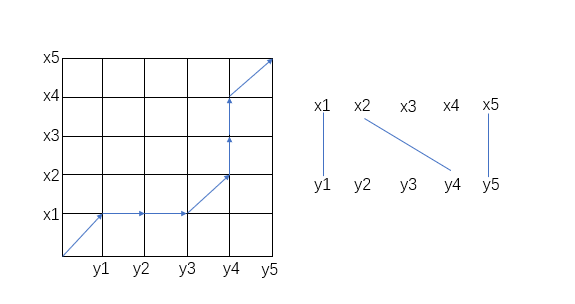
\includegraphics[scale=0.6]{image/connect2.png}
	\caption{构造图}\label{fig:connect2}
\end{figure}
按图构造方法如图所示

\input{src/LN18-DP-ZeroOneKnapsack.tex}
\input{src/Ln19-DP-ContextFreeGrammar.tex}
\input{src/Network-flows.tex}
\chapter{网络流应用之图像分割}

{\centering 本章简单介绍网络流在图像分割上的应用。}

\begin{definition}{背景知识}{}
	图像是可以看作由一个个像素组成的巨大图, 将像素一一用边连接起来, 则这些像素点会成为这个巨大图网络的顶点.
	一个图由前景和背景组成, 假设顶点上的值用 $a_i$ 表示, $ 0 \leq a_i \leq 1 $,  $a_i$ 趋近于 0 表示 $a_i$ 为图的背景, $a_i$ 趋近于 1 表示 $a_i$ 为图的前景, 并且设所有属于前景的顶点 $a_i$ 构成集合 A, 所有属于背景的顶点 $a_j$ 构成集合 B.
	假设边上的值用 $w_{ij}$ 表示, $w_{ij}$ 设为边的惩罚值, $w_{ij}$ 趋向于 0 表示“分离” (即 $w_{ij}$ 连接的两个点分别属于前景和背景), $w_{ij}$ 趋向于 1 表示“在一起” (即 $w_{ij}$ 连接的两个点都属于前景或者背景)
	设总的惩罚值为 $ A = \min\left(\sum_{i \epsilon B}a_i +  \sum_{i \epsilon A}(1 - a_j) + \sum_{i \epsilon A, j \epsilon B}w_{ij} \right) $
\end{definition}


\section{问题实例}
\subsection{问题描述}
\begin{itemize}
	\item 对于下面这个图,利用网络流求解该图前景和背景的最大可能
\end{itemize}

\begin{figure}[htb]
	\centering
	\includegraphics[scale=0.8]{image/Image-segmentation2.png}
	\caption{图片前景背景识别}\label{fig:image-seg-1}
\end{figure}

\subsection{思路描述}
\begin{itemize}
	\item 图形切割算法通过向图 G (V,E) 添加 S 点和 T 点,将图中所有的顶点,与 S 和 T 建立边,
	      如果一个点与 S 相连,则对应边的权值为该点的值 $a_i$, 如果一个点与 T 相连,则对应边的权值为1减去该点的值 $ 1 - a_j $。
	      可以得到下面这个图:
\end{itemize}

\begin{figure}[htb]
	\centering
	\includegraphics[height=4.5cm]{image/Image-segmentation3.png}
	\caption{图片前景背景识别}\label{fig:image-seg-2}
\end{figure}

\begin{itemize}
	\item   根据最大流最小割, 可以得到得到二分图的最大匹配, 可以得到集合A和B, 保证总的惩罚值 $ A = \min\left(\sum_{i \epsilon B}a_i +  \sum_{i \epsilon A}(1 - a_j) + \sum_{i \epsilon A, j \epsilon B}w_{ij} \right) $ 最小,
	      最小为 $(0.2 + 0.1) + (1 - 0.9) + (1 - 0.8) + 0.3 + 0.3 = 1.2 $, 而 A 和 B 分别对应图的前景和背景。
\end{itemize}

\section{问题扩展}
\begin{itemize}
	\item 假如一个图的前景不是一个整体,
	      而是有两个分开的部分,比如两只在两个不同位置的猫在一个图中。
	      这样一个算法能否将图像上的前景和背景分开?
\end{itemize}

\begin{figure}[htb]
	\centering
	\includegraphics[scale=0.6]{image/Image-segmentation1.png}
	\caption{图片前景背景识别}\label{fig:image-seg-3}
\end{figure}

\input{src/Ln26-P-NP.tex}

\bibliography{ref.bib}
\end{document}
